%sparsemul_result


%Versuch der Vergleichung von matlab,CPU-und GPU-Implementierung wird in Abb.\ref{sparse_ergebnis} und Tabelle \ref{tab_sparse_result}. ausgewiesen. Für 128-Diagonalmatix kann CUDA-Implementierung gegen CPU zu Faktor 9 erreichen.

Der Vergleich von Matlab, CPU- und GPU-Implementierung wird in
Abb.\ref{sparse_ergebnis} und
Tabelle \ref{tab_sparse_result} gezeigt.
Für eine 128-Diagonalmatix kann die CUDA-Implementierung (16x16)
einen Speedup-Faktor von 9 gegenüber der CPU erreichen.


\begin{figure}[htbp]
%\centering
%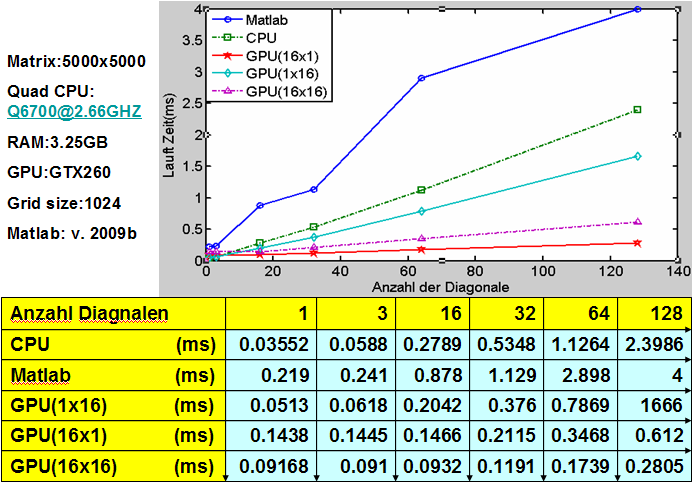
\includegraphics[width=3.5in]{../xby/pic//sparse_ergebnis}
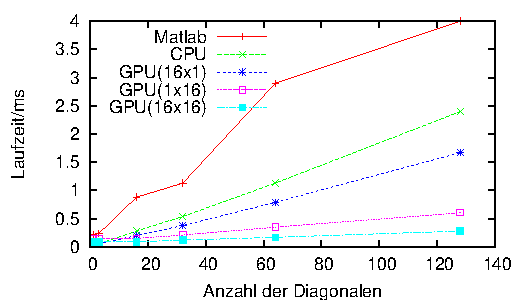
\includegraphics{../ausarbeitung/sparse/sparsegp.pdf}
\caption{Sparsematrix-Vektormultiplikation. Matrix 5000x5000, Quad CPU 2.66GHz, RAM 3.25GB, GPU GTX260, Grid size 1024}
\label{sparse_ergebnis}
\end{figure}


\begin{table}
%\begin{tabular}{|l|c|c|c|c|c|}
\renewcommand{\arraystretch}{1.3}
\caption{Ausführungszeiten der Sparsematrix-Vektormultiplikation in ms}
\label{tab_sparse_result}
\centering
%\begin{tabular}{|p{46pt}p{20pt}p{20pt}p{20pt}p{20pt}p{20pt}p{20pt}|}
\begin{tabular}{|l|r|r|r|r|r|r|}
%\begin{tabularx}{350pt}{1xxxxx}

\hline
Diagonalen& 1& 3& 16& 32& 64 &128\\


\hline
\hline
Matlab     &   0.219   &   0.241&   0.878  &  1.129 &  2.898  & 4\\
CPU        & 	0.036 &   0.059& 	0.279  &  0.535 &  1.126  & 2.399 \\
GPU(1x16)  & 0.051     &   0.062 &  0.204  &  0.376 &  0.787  & 1.666\\
GPU(16x1)  & 0.143     &	0.145 &	0.147  &  0.212 &	0.347 &	0.612\\

GPU(16x16)     & 0.092 &	0.091  &	0.0932 &	0.119&	0.174 &	0.281\\

\hline
\end{tabular}
%\end{tabularx}
\end{table}